
\documentclass[a4paper,12pt]{book}
\usepackage[font=scriptsize]{caption}
\usepackage[T1]{fontenc}
\usepackage[italian,english]{babel}
\usepackage[utf8]{inputenc}
\usepackage{graphicx}
\usepackage{grffile}
\usepackage{color}
\usepackage{float}
\usepackage{cite}
\usepackage{amsmath}
\usepackage{amssymb}
\usepackage{amsthm}
\usepackage{wasysym}
\usepackage{setspace}
\usepackage{algorithm}
\usepackage{algorithmic}
\usepackage{multirow}
\usepackage{listings}
\usepackage{url}
\usepackage[height=21.6cm,width=15cm,centering]{geometry}
\usepackage{tabularx}
\usepackage[super]{nth}

\usepackage[bookmarks=true,hyperindex,colorlinks=false,
            pdfborder={0 0 0},pdfstartview=FitH,pdfpagelayout=SinglePage,
            pdfauthor={Marco Edemanti},
            pdftitle={RASD WeatherCal},
            pdfsubject={}]{hyperref}

\title{RASD WeatherCal}
\author{Edemanti Marco}
\author{Polidori Paolo}

\begin{document}
\selectlanguage{english}
\definecolor{lightgray}{rgb}{.9,.9,.9}
\definecolor{darkgray}{rgb}{.4,.4,.4}
\definecolor{purple}{rgb}{0.65, 0.12, 0.82}
\definecolor{lightgreen}{rgb}{0.06,0.60,0.34}
\lstdefinelanguage{alloy}{
  keywords={t assert, pred, all, no, lone, one, some, check, run,
      but, let, implies, not, iff, in, and, or, set, sig, Int, int,
      if, then, else, exactly, disj, fact, fun, module, abstract,
      extends, open, none, univ, iden, seq,},
  keywordstyle=\color{blue}\bfseries,
  ndkeywords={class, export, boolean, throw, implements, import, this},
  ndkeywordstyle=\color{darkgray}\bfseries,
  identifierstyle=\color{black},
  sensitive=false,
  comment=[l]{//},
  morecomment=[s]{/*}{*/},
  commentstyle=\color{lightgreen}\bfseries,
  stringstyle=\color{red}\ttfamily,
  morestring=[b]',
  morestring=[b]"
}
\lstset{ %
  backgroundcolor=\color{white},   % choose the background color; you must add \usepackage{color} or \usepackage{xcolor}
  basicstyle=\footnotesize,        % the size of the fonts that are used for the code
  breakatwhitespace=false,         % sets if automatic breaks should only happen at whitespace
  breaklines=true,                 % sets automatic line breaking
  captionpos=b,                    % sets the caption-position to bottom
  commentstyle=\color{green},    % comment style
  deletekeywords={...},            % if you want to delete keywords from the given language
  escapeinside={\%*}{*)},          % if you want to add LaTeX within your code
  extendedchars=true,              % lets you use non-ASCII characters; for 8-bits encodings only, does not work with UTF-8
  frame=single,                    % adds a frame around the code
  keepspaces=true,                 % keeps spaces in text, useful for keeping indentation of code (possibly needs columns=flexible)
  keywordstyle=\color{blue},       % keyword style
  language=alloy,                 % the language of the code
  morekeywords={*,...},            % if you want to add more keywords to the set
  numbers=left,                    % where to put the line-numbers; possible values are (none, left, right)
  numbersep=5pt,                   % how far the line-numbers are from the code
  showspaces=false,                % show spaces everywhere adding particular underscores; it overrides 'showstringspaces'
  showstringspaces=false,          % underline spaces within strings only
  showtabs=false,                  % show tabs within strings adding particular underscores
  stepnumber=2,                    % the step between two line-numbers. If it's 1, each line will be numbered
  tabsize=2,                       % sets default tabsize to 2 spaces
}
 \begin{center}
    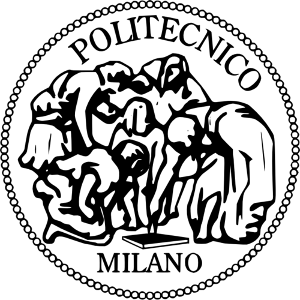
\includegraphics[width=4cm]{immagini/polilogo.png}
    \end{center}
\begin{center}

{\huge{\bf\uppercase {Requirements Analysis  \\and \vspace*{0.5cm} \\Specification Documents}}}


\end{center}
\vspace*{0.5cm}
\begin{center}
{\large Project of Software Engineering 2\\ \vspace*{0.5cm} \huge WEATHER-CAL}
\end{center}
\begin{flushright}
 \vspace*{9cm}

        {\bf Authors: }\\
        \vspace*{0.2cm}
            {\bf   {PAOLO POLIDORI} }\\
             \vspace*{0.3cm}
            {\bf   {MARCO EDEMANTI} }
    \end{flushright}

\doublespacing    
\tableofcontents
\vspace*{\fill}
\section*{Revisions}
\begin{tabularx}{\linewidth}{|r|X|}
  \hline Date & Comments\\
  \hline Nov, \nth{16}, 2014 & First version\\
  \hline Dec., \nth{7}, 2014 & Revision of Class Diagram\\
  \hline
\end{tabularx}

\chapter{Introduction} \label{cap:cap1}

\section{Purpose}
The purpose of this document is to present a description of WheaterCal system. It will explain the features of the system, the interfaces of the system, what the system will do and the constraints under which it must operate.
This document is intended for both the stakeholders and the developers of the system.
Stakeholders of the system are the client, which is our teacher and their assistants, composing the group that will evaluate our project, the testers, which are a team with our same project and our same tasks and the developers, which are the authors of this document.

\section{Scope}
We want to project and implement WheaterCal. The aim of this project is to develop a system that offers an online calendar in which user can schedule their events according to the weather conditions.\\ A registered user can create, delete and update an event and moreover he should provide information about where and when this event will take place and information about the invited user.
Once the event is created the system should provide to its creator the weather forecast information regarding the scheduled day, and most of all it should notify a bad weather condition one day in advance to all the participants.\\
Also a user is able to make his/her calendar visible to all other registered user showing them only the time slots in which they are busy without letting know the event information unless either the event is public.
In addition in case of bad weather, three day before the scheduled data of an event, the system will inform the event's owner and propose to him the closest sunny day.

\section{Glossary}
\begin{tabularx}{\linewidth}{|r|X|}
  \hline  {\bf Anonymous User} & People who access the system but didn't authenticate\\ 
  \hline  {\bf Registered User} & People who both registered to the platform and logged in. Sometimes referred to as "User"\\ 
  \hline  {\bf Platform, System} & The WeatherCal application\\
  \hline  {\bf Bad Weather}&  Undesired conditions for an event to take place basing on the event owner's choices\\
  \hline  {\bf Notification} & A message that arrives to the user in dedicated area, which can be easily identified by the user at first sight\\
  \hline  {\bf Event owner} & The user who created the event and for which is responsibile of the organization\\
  \hline  {\bf Event invited} & A user invited to an event for which can decide if he wants to be a participant or not\\
  \hline  {\bf Event participant} & A user invited to an event for which decided to participate\\
  \hline  {\bf Event} & An occurrence, which was inserted in the system which should happen in a certain date and a certain time\\
  \hline  {\bf Calendar} & The set of all the events for a user, shown in a per-month view\\
  \hline
\end{tabularx}\\
\section{References}
IEEE,{\it IEEE Std 830-1998,IEEE Recommended Practice for Software Requirements Specifications},  IEEE Computer Society 1998

 
\chapter{Overall Description} \label{cap:cap2}
\section{System Environment}
WeatherCal is a stand alone software made from scratch. It is a Web application that allows the registered users to manage their schedule basing on the weather conditions. The users are also able to invite people to their event and to publicize their event.  
The system is even capable of notifying the users, as they log on to the system, if the weather forecast for the event is not the desired one.
The target of this software is, therefore, to give the users a tool for schedule their events smartly, giving the possibility to change preferences as the weather forecast changes.
\subsection{Actors}
Actors in the system are mainly the people registered into the web application. They will be referred as Registered Users.
Whoever is not yet registered on the platform will be an actor for the system too and it will be identified as an Anonymous  Users.
No administration is required since the system is not intended for illicit purposes and this is a policy of the platform, plus no conflict among users can occur since the only allowed interactions are the invite to an event and a participation to an event (in which other people partecipate).
\subsection{Scenarios}
\begin{itemize}
\item Maggie creates an event for her daughter's birthday, which will be in their garden. She invites all her friends telling them to join the event on WeatherCal to be sure that the forecast will be graceful for that day. Three days before the birthday, Maggie logs in two days before the event and she discovers it will be cloud but she still hopes it won't rain on that day. The day before the event Judith, Maggie's friend, is notified that it could be rainy for the birthday as she logs into the system. Anyway Maggie decides she won't posticipate the birthday. In the end that day was rainy, except for the afternoon, exactly for the birthday, and everything went fine.
\item John wants to go cycling but right now the forecast is not so optimistic, so he decides to use WeatherCal to find the best day for doing so. The platform suggests him that he should go on Monday afternoon, so he plans to do that. Saturday he logs in and discovers that it will be windy on Monday, infact the system suggests him to go cycling on Wednesday and John chooses to do what the system suggests him. In the end he went cycling and the weather was perfect.
\item Beth wants to have a picnic with her friends in two weeks, so she creates an event on WeatherCal when the temperature should be the hottest and there should be no clouds in the sky. Three days before she logs in discovering that for the next two weeks there will be bad weather conditions. She decides so to invite her friends at home for having a launch together.
\end{itemize}
\section{Functional Requirements}
The system allows the users to partecipate in various scenarios:
\begin{itemize}
\item Log on to and log out from the platform.
\item Create, Modify, Delete an event.
\item Invite other users.
\item Manage participations (accept, refuse, ...).
\item Manage event visibility (decide if an event's infos should be accessible only by its invited). 
\item View other users' profiles (see other users's calendar only if it's set public and see the events' details if they mark public too or you are invited to them)
\end{itemize}
The system is the leading actor in:
\begin{itemize}
\item {Warning all the participants to an event which will occur the following day that there will be bad weather conditions if so.} 
\item Notify to an event's owner three day before the scheduled data that there will be bad conditions for it suggesting the closest available sunny day.
\end{itemize}
The Anonymous Users are only able to:
\begin{itemize}
\item Sign Up in to the Platform.
\end{itemize}
\section {Goals}
The WeatherCal system should offer and fulfill these main features:
\begin{itemize}
\item A simple management for the users' agendas
\item A swift way to schedule an event according to the weather forecast 
\item Invite other registered users to an event
\item Preserve the privacy of the users since only the user himself can make their info visibile to everyone.
\end{itemize}
\section{Non Functional Requirements}
\subsection{User Interfaces}
The WeatherCal system is a Web application intended to be used trough a desktop device.  Its interface is designed in a simple way so that  the user can either easily understand what the system can offer to him and reache all the main features of the system from a unique view.\\
Once that a user logs in to the system trough a defined web page he is redirected to the main page. This page is divided in two portions. The left one, which occupies the largest portion of the page, displays a monthly calendar in which the user manages its events while the right one shows the weather forecast for the following days and also shows the closest events.\\In the figure~\ref{fig:mockup} is shown a first sketch of the main user's page.\\ \\  
 \begin{center}
 \begin{figure}
    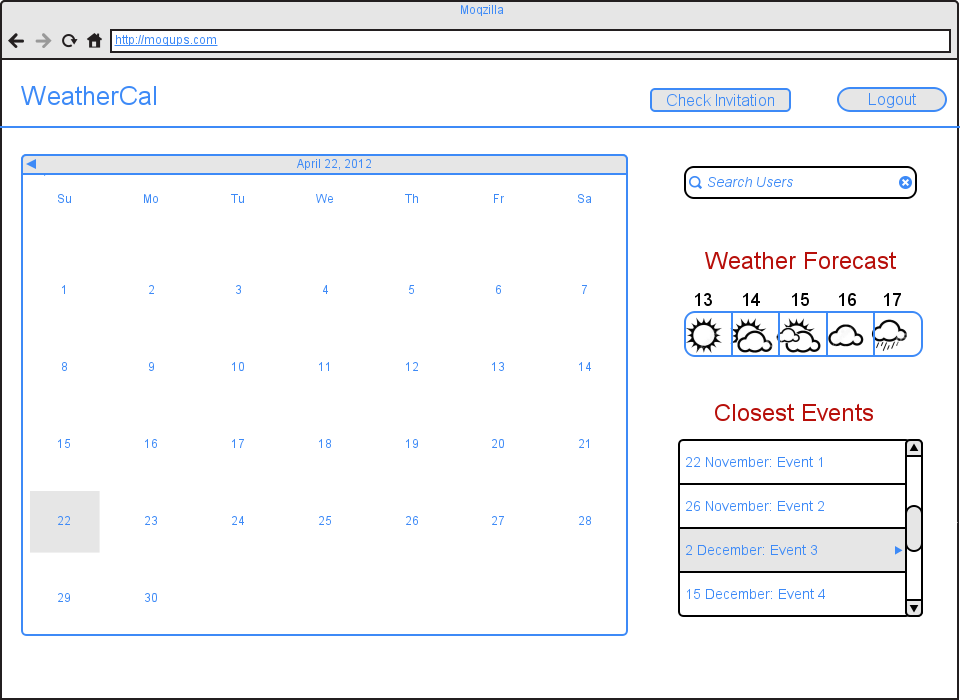
\includegraphics[width=0.9\textwidth]{immagini/UserPage.png}
    \caption{Main Page's MockUp}
     \label{fig:mockup}
     \end{figure}
    \end{center}
\subsection{Performance}
The system offers the users the possibility to use it without major slowdowns. Multiuser usage is allowed and it can be bore by the server application under reasonable conditions, basing on the server hardware.
\subsection{Security}
The system relies on HTTP protocol for transferring data over the Internet, so information sent both from the user to the server and vice-versa will be exposed to possible man-in-the-middle attacks. Unless this issue data stored on the server will be accessible only if valid credentials are provided and there is no possibility for a user to bypass privacy constraints, i.e. users will not be able to see non-public events of other users and modify events for which they are not owners. This will be accomplished from the server by performing checks on the data requested by the client (authorization politics).
\chapter{System Modeling} \label{cap:cap4}
\section{UML Diagrams}
\subsection{Use Case Diagrams}
\subsubsection{Event Management}
The use case in figure~\ref{fig:eventusecase} shows how a user can manage his agenda. After he logs into the platform he will see his calendar and being able to see schedule of his events. This event can be modified and so deleted or if the user is the event's owner he can invite other users.
 \begin{center}
 \begin{figure}[H]
    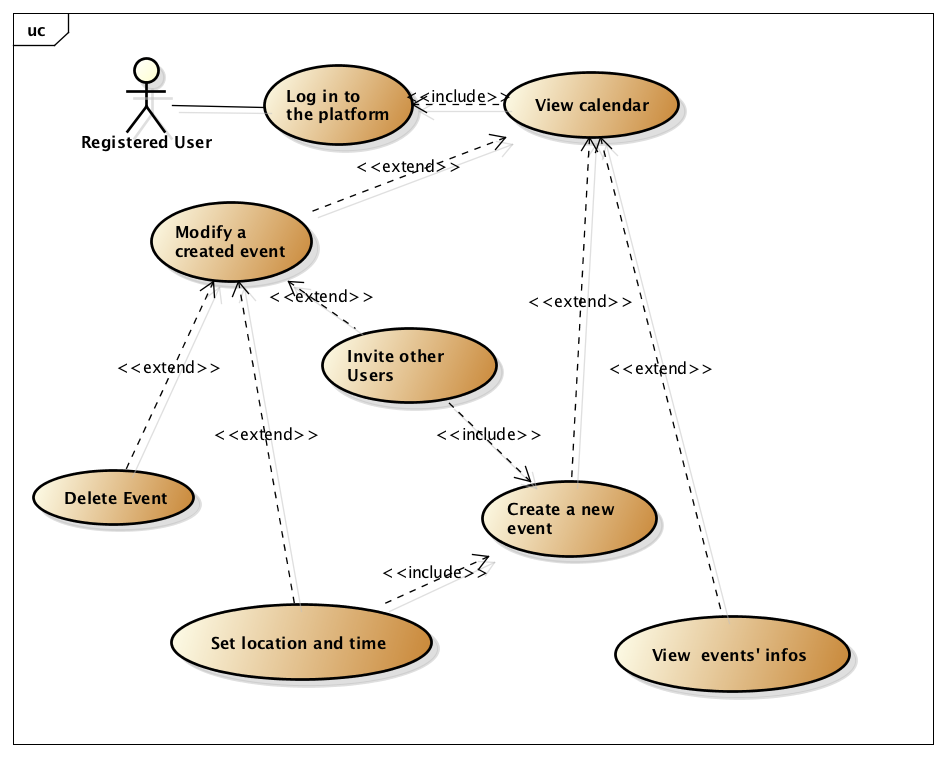
\includegraphics[width=1\textwidth]{../UMLDiagram/use_case/EventManagmentUseCase/EventManagment.png}
    \caption{Event Management Use Case}
     \label{fig:eventusecase}
     \end{figure}
   \end{center}  
The use case in the shows how a user can manage his agenda. After he logs into the platform he will see his calendar and being able to see schedule of his events.This events can be modified and so deleted or if he is the event's owner he can invite other users.This use case show how a user can manage his agenda. After he logs into the platform he will see his calendar and being able to see schedule of his events.This events can be modified and so deleted or if he is the event's owner he can invite other users.
\subsubsection{Invitation}
The use case in figure \ref{fig:invitusecase} explains what the user can do when he receive an invitation to an event from an other user. Once he get the notification he can either see the event's info and accept or decline the invitation.\\\\\\
 \begin{center}
 \begin{figure}[H]
    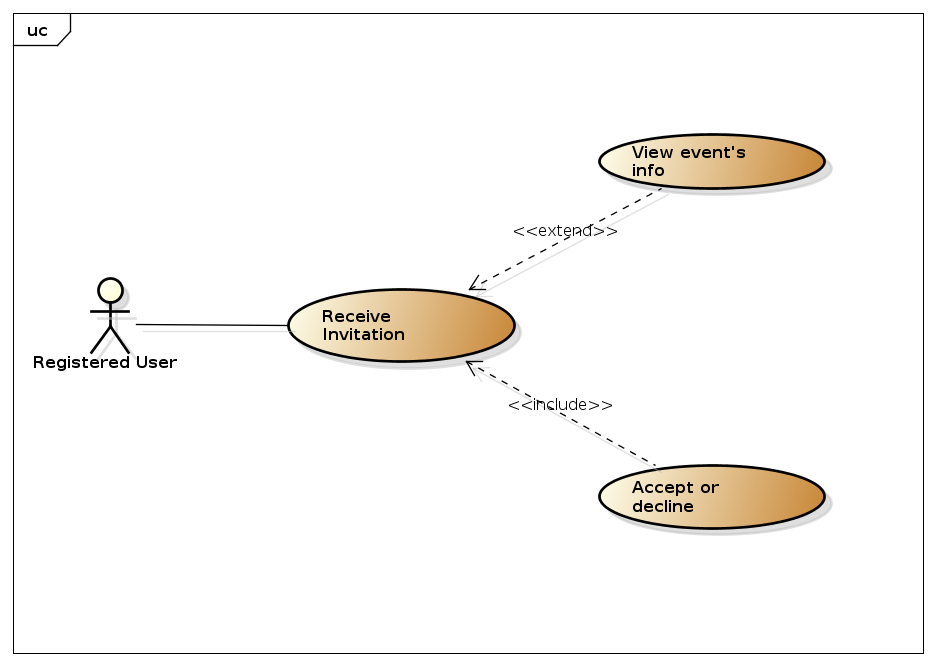
\includegraphics[width=1\textwidth]{../UMLDiagram/use_case/Invitation/Invitation.png}
    \caption{Invitation Use Case}
     \label{fig:invitusecase}
     \end{figure}
   \end{center}  
\subsubsection{View other users' profiles}
The use case in figure \ref{fig:otherprofileusecase} shows how an user can reach the profile of an other user and view his agenda. After he logs in to the platform he will be able to search an user and see his profile, but he will be authorized to see the other user's calendar only if it is set as public by its owner.   
 \begin{center}
 \begin{figure}[H]
    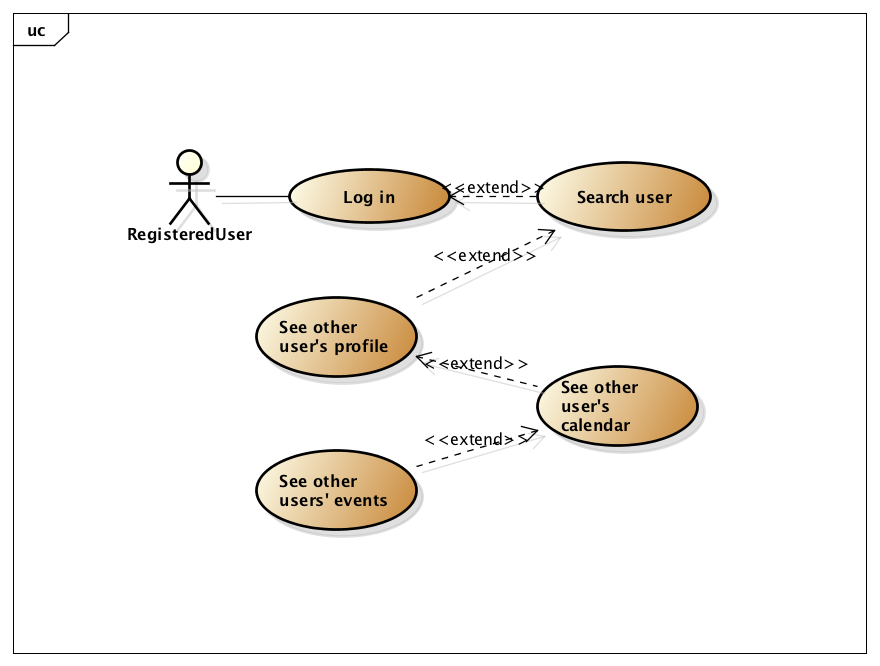
\includegraphics[width=1\textwidth]{../UMLDiagram/use_case/ViewOtherProfiles/UseCaseDiagram0.png}
    \caption{See Other User Profile Use Case}
     \label{fig:otherprofileusecase}
     \end{figure}
   \end{center}  
\subsubsection{Bad Weather}
The use case in figure \ref{fig:otherprofileusecase} explains how an user can behave when he get notified by the platform in case of bad weather condition. Whenever he receives a bad weather notifications the user can act in two different way. If he's the event's owner he can delete the event or modify the event's location while if he's an event's participant he can only manage his event's participation.
 \begin{center}
 \begin{figure}[H]
    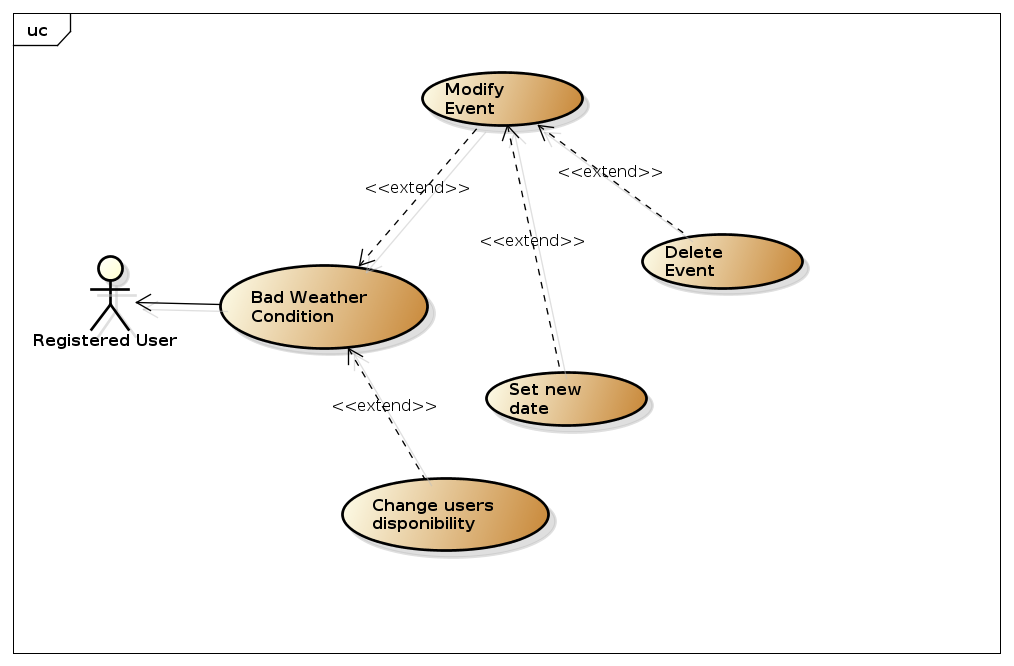
\includegraphics[width=1.1\textwidth]{../UMLDiagram/use_case/BadWeather/BadWeather.png}
    \caption{Bad Weather Use Case}
     \label{fig:badweatherusecase}
     \end{figure}
   \end{center}  
\subsection{Class Diagrams}
Once that the requirements of our platform have been defined we are able to compose the class diagram  of the system,as shown in figure ~\ref{fig:classdiagram}.
\begin{center}
 \begin{figure}
    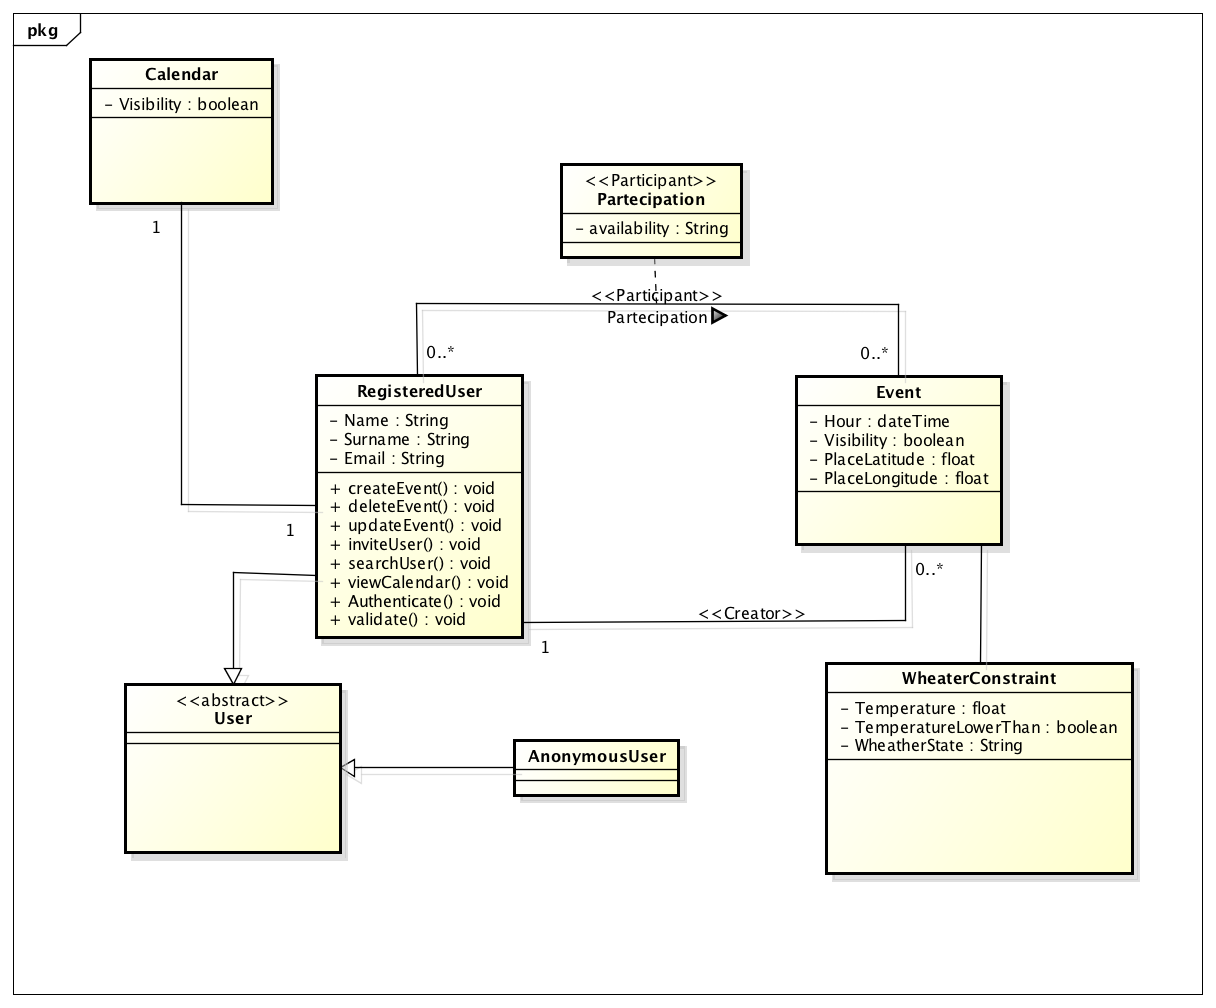
\includegraphics[width=1\textwidth]{../UMLDiagram/class/WeatherCalClassDiagram/ClassDiagram0.png}
    \caption{Class Diagram}
     \label{fig:classdiagram}
     \end{figure}
   \end{center}  
\subsection{State Diagrams}
\subsubsection{Invitation}\label{sssec:invitationstate} 
In figure \ref{fig:invstatediagram} the state diagram of an invitation to an event is shown.
 \begin{center}
 \begin{figure}[H]
    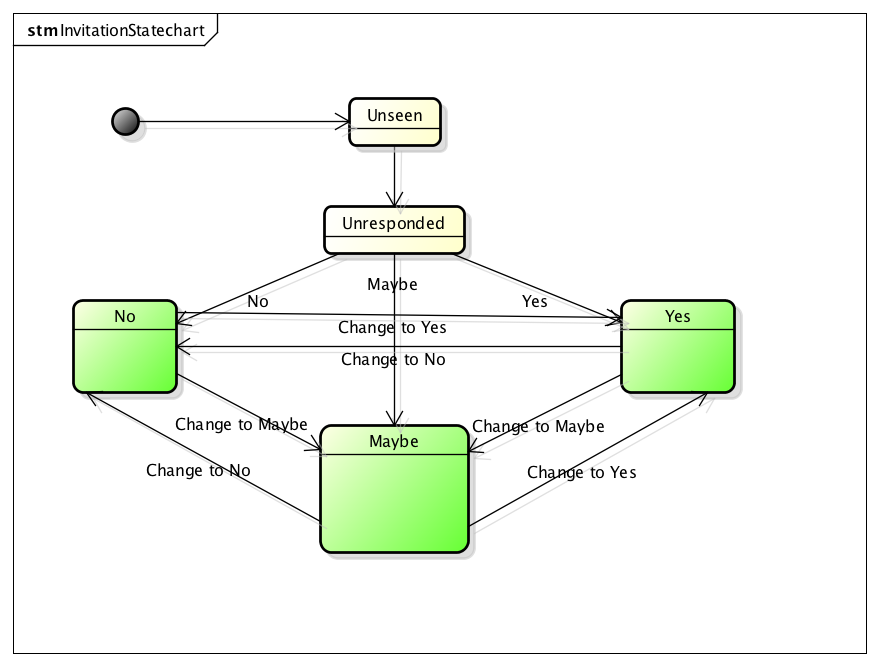
\includegraphics[width=1\textwidth ]{../UMLDiagram/InvitationStatechart/InvitationStatechart.png}
    \caption{Invitation State Diagram}
     \label{fig:invstatediagram}
     \end{figure}
   \end{center}
As the event owner invites a user, an invitation is created, having an unknown participation, which is defined by the first state. When an invitation is in this state means that an invitation for a user to an event has been made, but he didn't seen that yet. When he logs onto the platform the state of the invitation changes to unresponded, since it has been shown to the user, but he didn't choose what to do yet. As the user responds to the notification, the state of the invitation becomes definite, so in can be "Yes", "No" or "Maybe". This will not necessarily happen when the user is notified about an invitation. After the user chosen what to do, he can then change his participation among the defined states (marked in green), and consequentially the state, until the event has ended. Infact, after the end of the event the modification of the participation will be disallowed.
 \subsection{Sequence Diagrams}
\subsubsection{User Registration}
Figure \ref{fig:regseqdiag} shows the process for the registration of a new user into the WeatherCal platform. As a user accesses the system, it will prompt it either to login or to register to the system. If the user chooses the latter this is what happens.
\begin{center}
 \begin{figure}[H]
    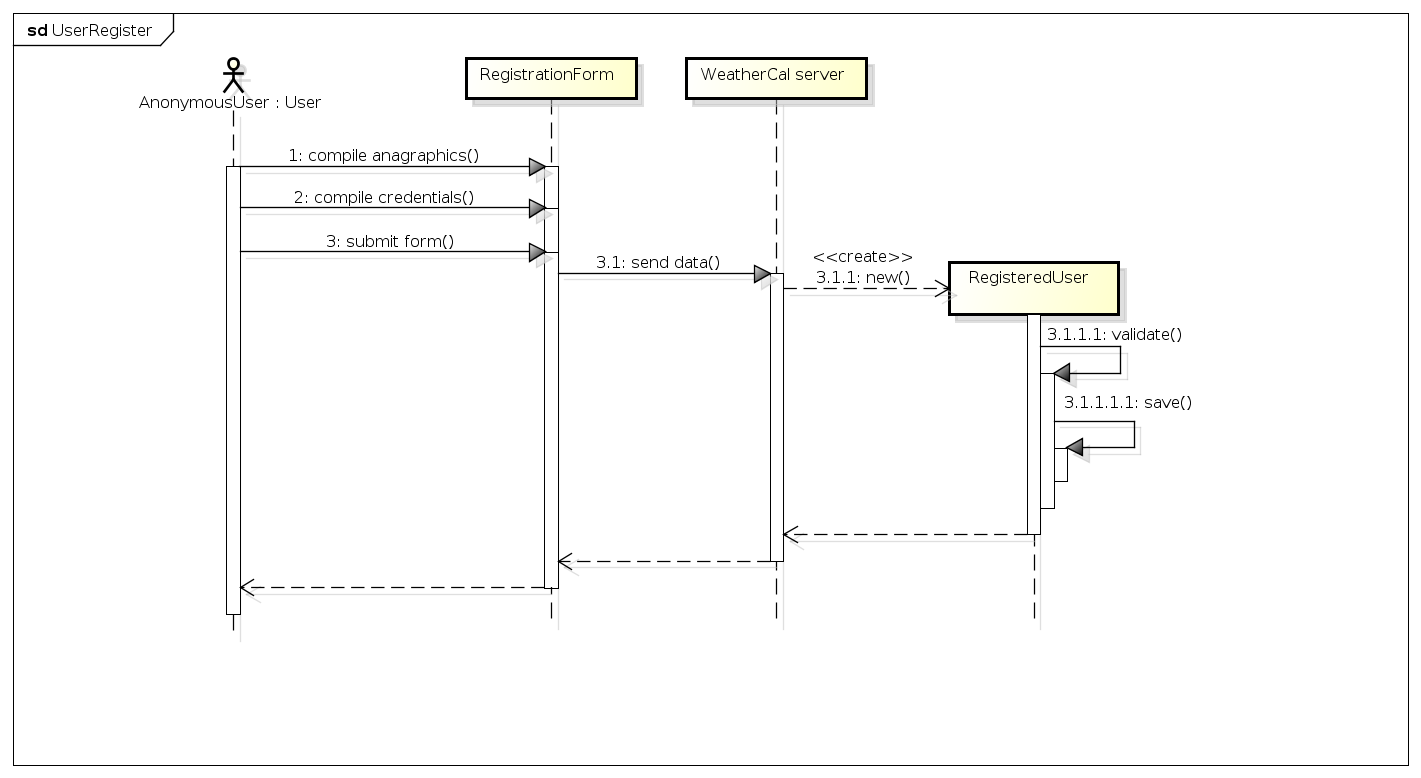
\includegraphics[width=1\textwidth]{../UMLDiagram/sequence/UserRegister/UserRegister.png}
    \caption{Sequence diagram of user registration}
     \label{fig:regseqdiag}
     \end{figure}
   \end{center}  
The user will see a registration form in which he will input his data and the credentials he wants to use for accessing the system. As the user submits the form and data is sent to the server the validation occurs. It can happen that, for instance, a new user chooses an already taken nickname, or he registers with an email which is yet on the system. These cases will cause an exception to be thrown and an error to be displayed to the user. However, in this diagram, the case in which the validation succedes is represented. After that, the user data will be stored and the credentials can be used for authentication purposes.
\newpage
\subsubsection{Login}
The diagram represented in figure \ref{fig:logseqdiag} describes the login phase for a registered user in the system. As the user enters the platform the login form is showed him and this process begins.
\begin{center}
 \begin{figure}[H]
    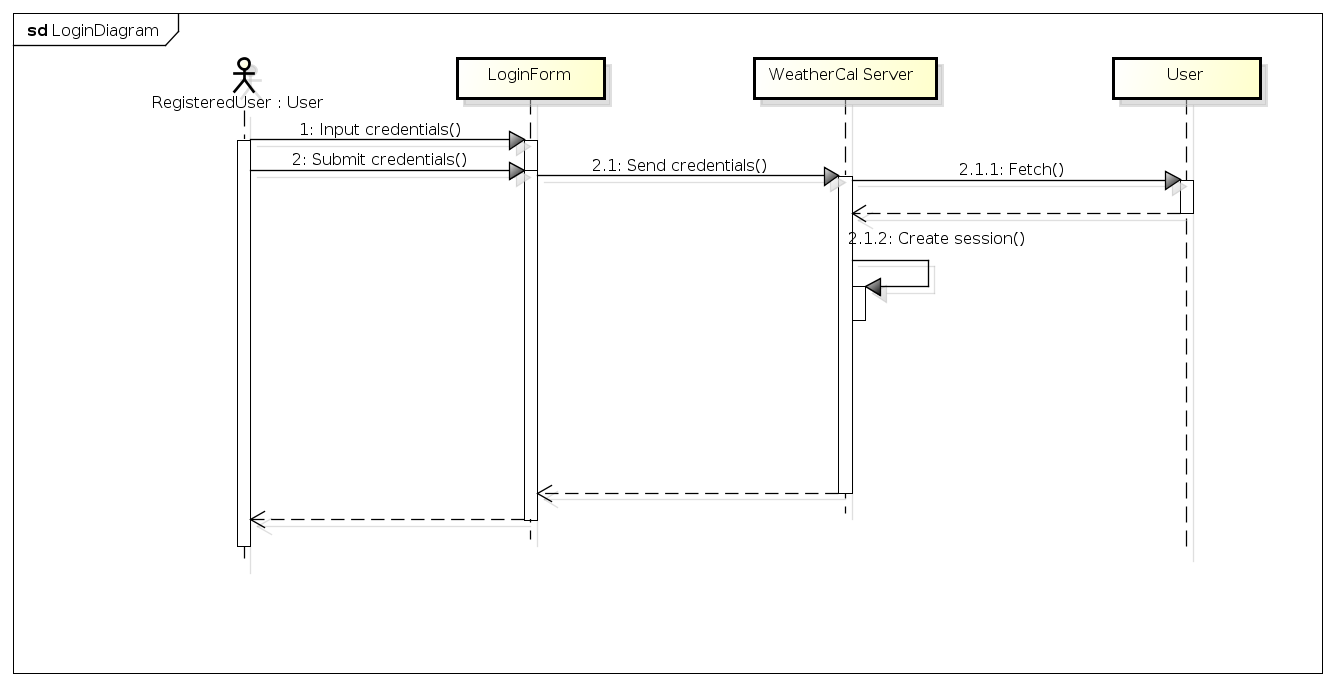
\includegraphics[width=1\textwidth]{../UMLDiagram/sequence/LoginDiagram/LoginDiagram.png}
    \caption{Login Sequence Diagram}
     \label{fig:logseqdiag}
     \end{figure}
   \end{center}
First of all the user fills the form with his username and password, which he decided during the registration. As he submits his credentials they are sent to the server. The server then tries to fetch a User from the persistance, but if not found an exception will be thrown and the user will be notified about the wrong data inputed. In this sequence diagram, however, the credentials in the form are supposed to be valid, and so the user will be authenticated to the system and identified by his own session, so he won't need to login for every action he wants to perform.
\subsubsection{Event creation}
In the diagram represented in figure \ref{fig:createseqdiag} the user will create a new event and customize it as he wants. The user will be able to start this procedure by clicking on the calendar and choosing to create a new event, making a form for inputing event data appear.
\begin{center}
 \begin{figure}[H]
    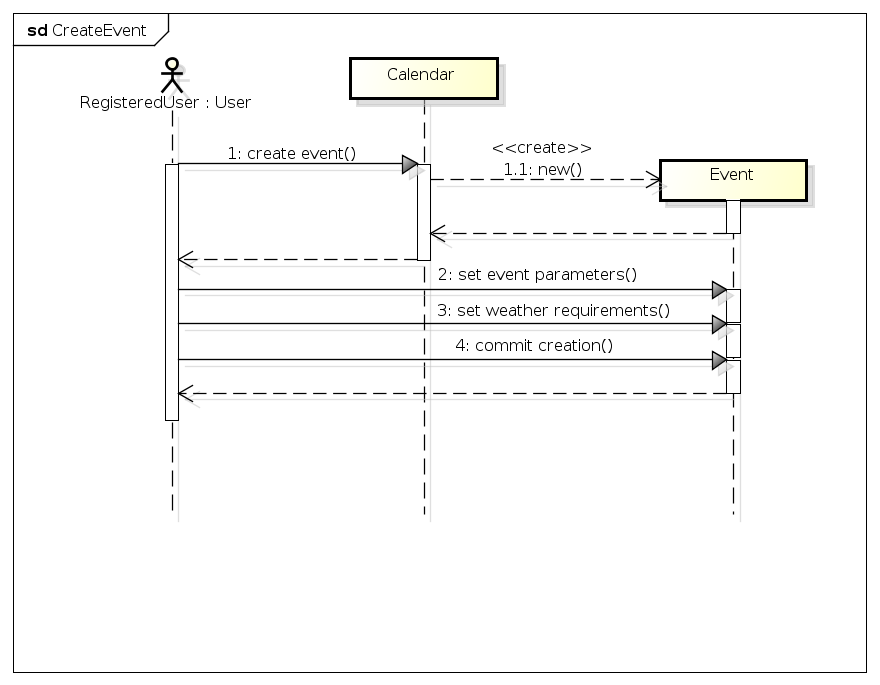
\includegraphics[width=1\textwidth]{../UMLDiagram/sequence/CreateEvent/CreateEvent.png}
    \caption{Create Event Sequence Diagram}
     \label{fig:createseqdiag}
     \end{figure}
   \end{center}
As the form opens the user is able to set all the parameters he desires for the event, such name, place, time, visibility and so on. He will be also able to set the constraints he prefers for the event, i.e. a temperature higher than a certain value, or that the sky must be sunny. After that all the required fields are filled, inputed data is valid and the user submits the form, the event is created and shown in his calendar. If data is not valid or required fields were not filled, an appropriate exception will be thrown and the user will be warned.
\subsubsection{Event modification}
When a user selects an event he will be able to enter a form in which he can modify certain parameters. This behaviour is described in figure \ref{fig:modseqdiag}.
\begin{center}
 \begin{figure}[H]
    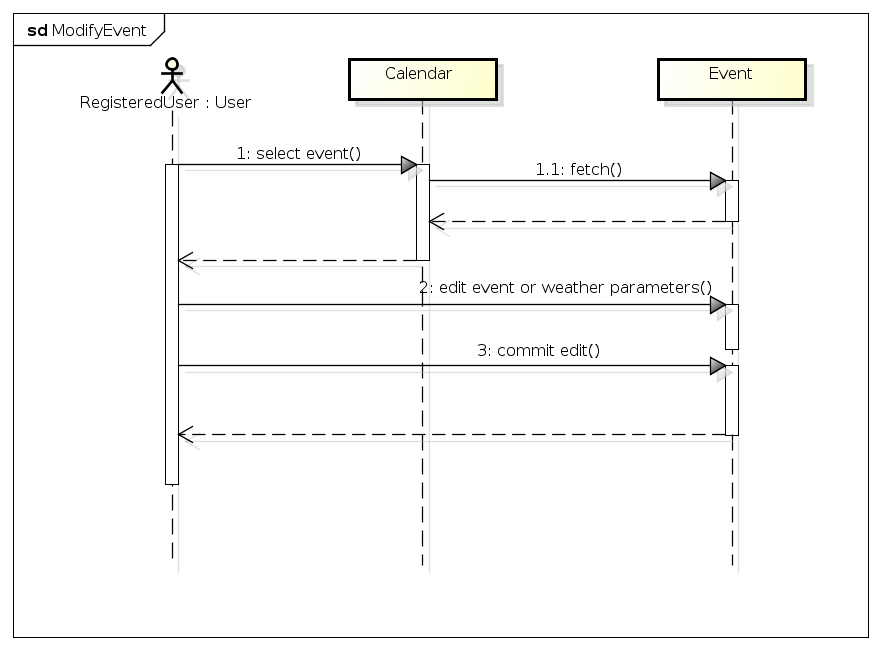
\includegraphics[width=1\textwidth]{../UMLDiagram/sequence/ModifyEvent/ModifyEvent.png}
    \caption{Sequence Diagram of event's modification}
     \label{fig:modseqdiag}
     \end{figure}
   \end{center}
When a modification of an event is requested, it is fetched and displayed to the user, in a form similar to the creation form. He can so change whatever is shown as editable and then, when he confirms the modification, they are saved serverside and showed both to his and to the invited users' calendars.
\subsubsection{Event deletion}
In this diagram, shown in figure \ref{fig:delseqdiag}, the process with which a user deletes an event is described.
\begin{center}
 \begin{figure}[H]
    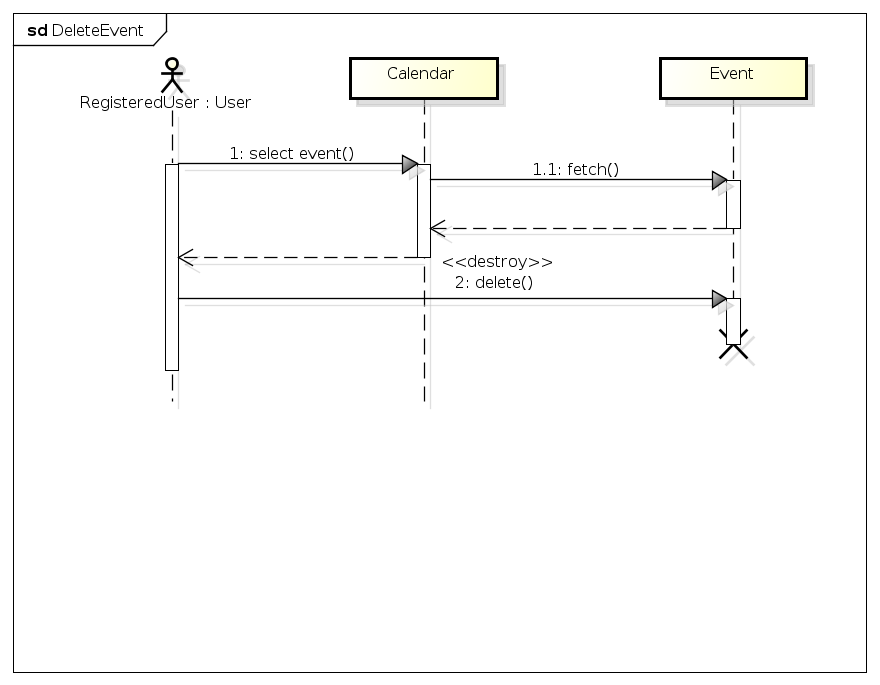
\includegraphics[width=1\textwidth]{../UMLDiagram/sequence/DeleteEvent/DeleteEvent.png}
    \caption{Sequence Diagram of event's deletion}
     \label{fig:delseqdiag}
     \end{figure}
   \end{center}
Starting from the calendar, a user selects an event for which is owner, and clicks the deletion button. The first selection makes the event to be loaded and then the click on the button, makes it to be deleted. Thus, this last action must be performed by the owner of the event, and an authorization check must be performed during the deletion, throwing an exception and so an error if a user tries to delete an event for which he is not the owner.
\newpage
\subsubsection{Invitation}
Figure \ref{fig:invitseqdiag} shows the steps for inviting a user to an event. This process begins with a user selecting an event for which he is the owner.
\begin{center}
 \begin{figure}[H]
    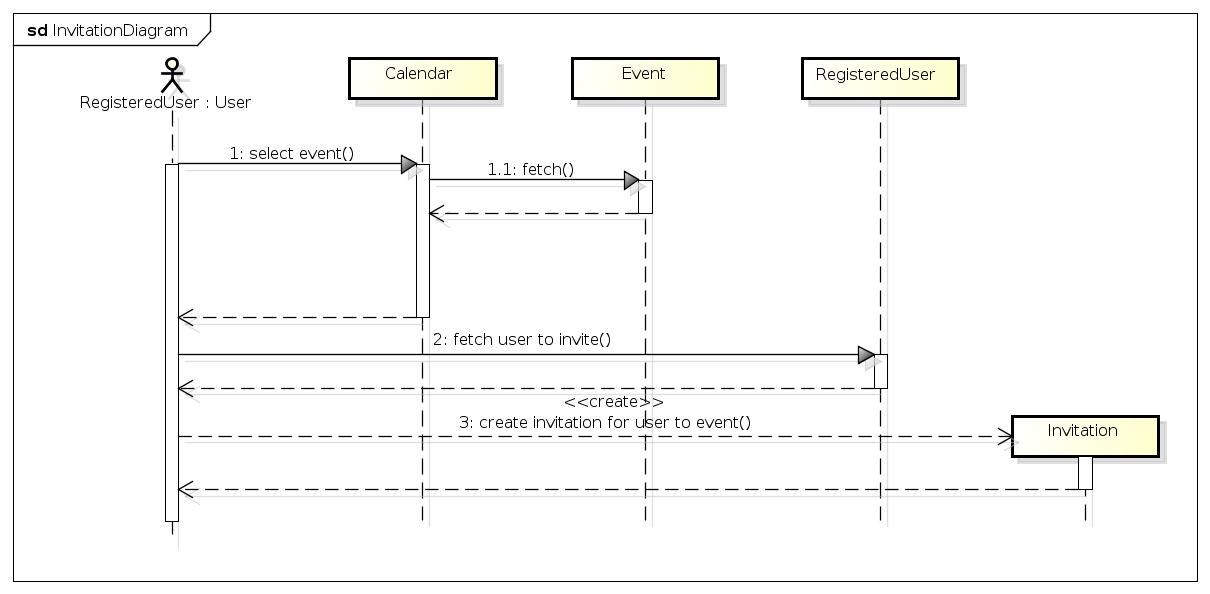
\includegraphics[width=1\textwidth,height=1\textwidth]{../UMLDiagram/sequence/InvitationDiagram/InvitationDiagram.png}
    \caption{Sequence Diagram of an invitation}
     \label{fig:invitseqdiag}
     \end{figure}
   \end{center}
As he does so, the event is loaded and the user is able to look for people to invite to his event. As the users are selected, and the modification is confirmed, the invitation are created. This makes the invitation to be notified at the invited users' next login. Anyway this process can end with an error, and then an exception, when a user tries to invite people for an event for which he is not owner. This will be not allowed as an authorization politic and so any invitation will be created.
\newpage
\subsubsection{Invite notification}
Here the invite notification is described, and shown in figure \ref{fig:notseqdiagr}. The behaviour described in the former paragraph asynchronously triggers this procedure.
\begin{center}
 \begin{figure}[H]
    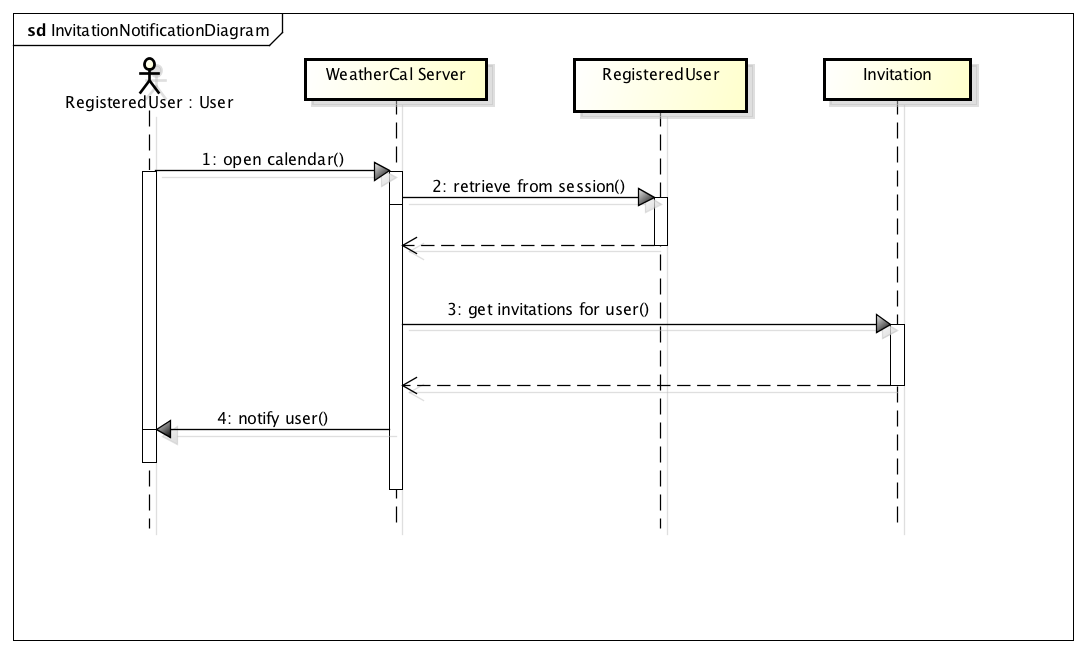
\includegraphics[width=1\textwidth,height=1\textwidth]{../UMLDiagram/sequence/InvitationNotificationDiagram/InvitationNotificationDiagram.png}
    \caption{Sequence Diagram of an invitation's notification}
     \label{fig:notseqdiagr}
     \end{figure}
   \end{center}  
As the user logs onto the platform and his calendar starts to be loaded he can notice that he was invited to an event (or more than just one). This happens because as the server notices that that user opens the calendar, it looks for unseen notifications. If it finds at least one notification it shows the user a message that informs him about that, giving him the possibility to choose what to do or even ignore that notification. 
\subsubsection{Modify participation}
In the figure \ref{fig:modpartseqdiag} a description of what happens when the user changes his mind about the participation to an event is illustrated.
\begin{center}
 \begin{figure}[H]
    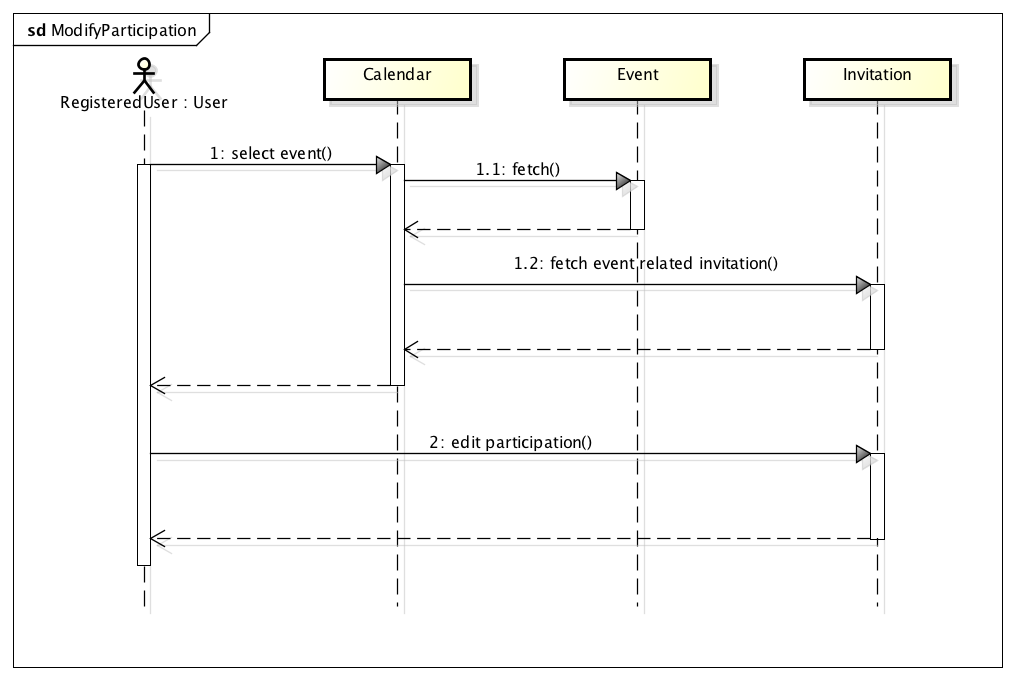
\includegraphics[width=1\textwidth]{../UMLDiagram/sequence/ModifyParticipation/ModifyParticipation.png}
    \caption{Modify participation Sequence Diagram}
     \label{fig:modpartseqdiag}
     \end{figure}
   \end{center}
As he selects an event from his calendar, its data is fetched and, in case he is an invited to the event, the invited is fetched too. In this case he will be able to change the state of the participation, as described in the related diagram in section \ref{sssec:invitationstate}. As he modifies it the change is reported onto the server. If invalid values for the state are sent to the server, it will throw an exception and no modification will occur. 
\section{Alloy}
We use Alloy Analyzer to figure out if our Class Diagram was designed in a consistent way so that even our system will be implemented in a consistent style.\\
Below are reported the code used to represent our system and some models generated by the Alloy Analyzer tool.
\subsection{Code}
\singlespacing
\begin{lstlisting}[frame=single,caption=Alloy Analyzer code, label=list:alloycode]
//SIGNATURE
sig RegisteredUser{
calendar:one Calendar
}
sig Invitation{
Guest: some RegisteredUser,
event:one Event
}
sig WeatherConstrain{
}
sig Calendar{
}
sig Event{
 Owner:one RegisteredUser,
 constrain:one WeatherConstrain
}
//FACTS
fact calendarConstrain{
//the number of Calendar must be equals to the RegisteredUser
#Calendar=#RegisteredUser
//two or more RegisteredUser cannot refer to the same calendar
no disj r1,r2:RegisteredUser | r1.calendar=r2.calendar
}
fact eventConstrain{
//the number of Invitation must be equals to Event
#Event=#Invitation
//each event refer to a different weather constrain
#WeatherConstrain=#Event
no disj e1,e2:Event | e1.constrain=e2.constrain
}
fact invitationConstrain{
//two or more Invitation cannot refer to the same event 
no disj r,p:Invitation | p.event=r.event 
//the owner of an event cannot receive the invitation of its event
all  disj e:Event , i1: Invitation | i1.event=e implies e.Owner not in i1.Guest
}
//ASSERTION
assert oneCalendarforUser{
no disj r1,r2:RegisteredUser | r1.calendar=r2.calendar
}
//check oneCalendarforUser
assert  ownerNotReceveir{
all  disj e:Event , i1: Invitation | i1.event=e implies e.Owner not in i1.Guest 
}
//check ownerNotReceveir
assert oneInvitationforEvent{
no disj r,p:Invitation | p.event=r.event and p.Guest = r.Guest
}
//check oneInvitationforEvent
assert onecal{
#Calendar=#RegisteredUser
}
//check cal
assert oneConstrain{
no disj e1,e2:Event | e1.constrain=e2.constrain
}
//check oneConstrain
pred show(){} 
run show 
\end{lstlisting}
\doublespacing
As shown in figure~\ref{fig:asser} the {\it Assertion} hence even the {\it Facts} made in the listing~\ref{list:alloycode} are verified because no counterexample was found therefore our system is designed in a coherent way.
\begin{center}
 \begin{figure}[H]
    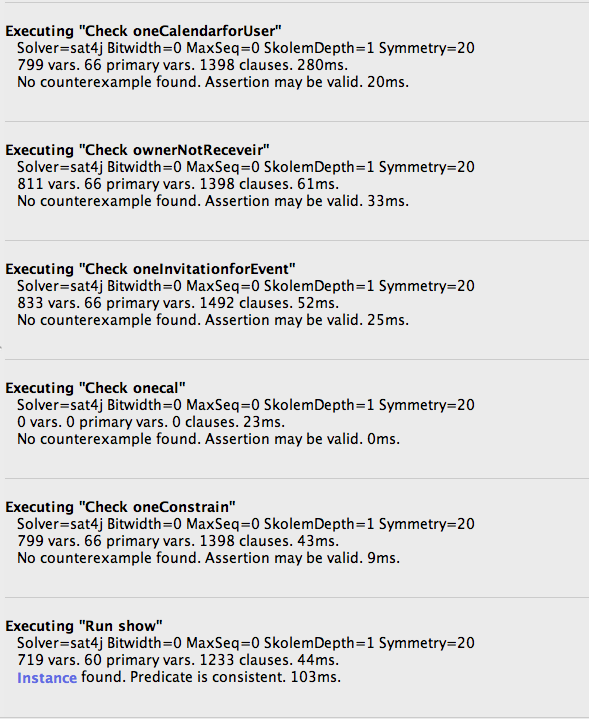
\includegraphics[width=0.6\textwidth]{../Alloy/checkassert.png}
    \caption{Assertion verified}
     \label{fig:asser}
     \end{figure}
   \end{center} 
\newpage
\subsection{Model generated}
In this section are reported some of the various scenarios representing the model of our system.
\subsubsection{Interaction between all users}
The model in figure ~\ref{fig:allint} represents a scenario in which all the users are both event's owner and event's participant. As we can observe from the model an  event's owner cannot be a guest of the invitation and all the event should refer to one at only one owner.
\begin{center}
 \begin{figure}[H]
    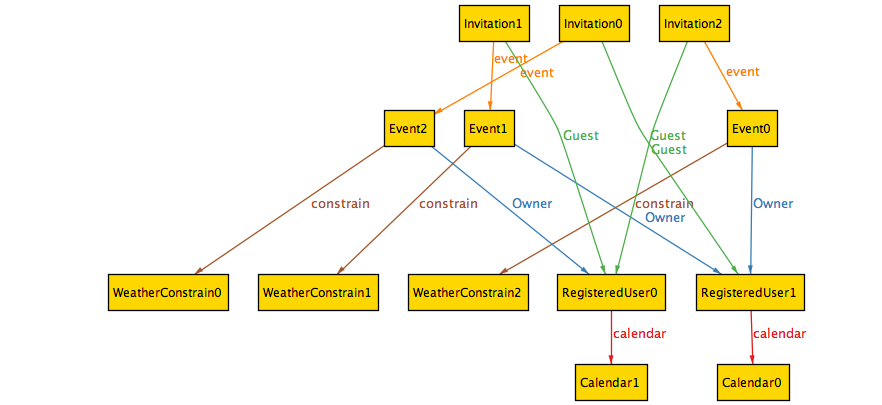
\includegraphics[width=1\textwidth,height=0.5\textwidth]{../Alloy/allInteration.png}
    \caption{All user interaction model}
     \label{fig:allint}
     \end{figure}
   \end{center} 
\subsubsection{Interaction only between a few users}
The model in figure ~\ref{fig:mixint} represents a scenario in which only some users are interacting and other users are not participating at none of the scheduled event.
\begin{center}
 \begin{figure}[H]
    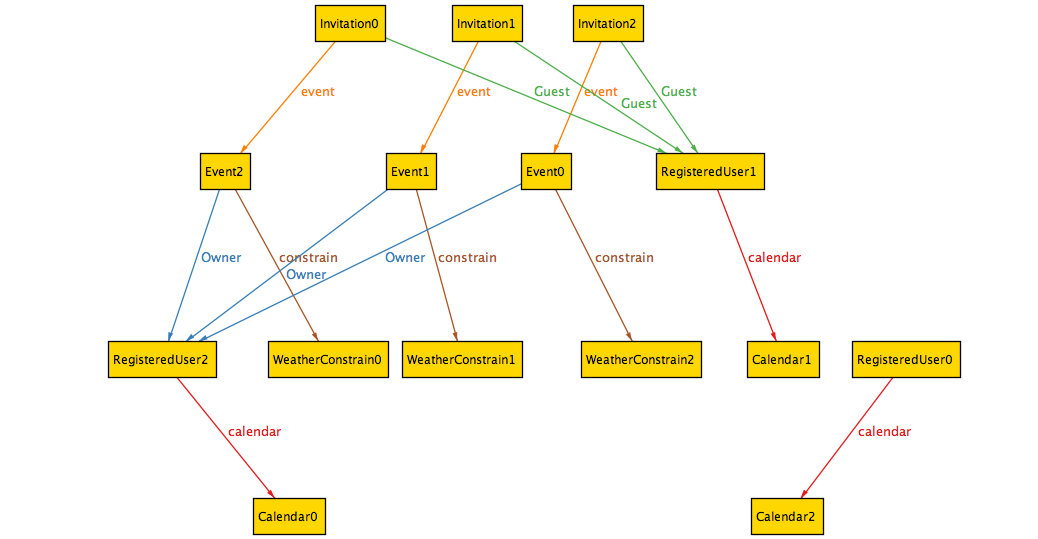
\includegraphics[width=1.1\textwidth,height=0.7\textwidth]{../Alloy/mixInt.png}
    \caption{Mixed interaction model}
     \label{fig:mixint}
     \end{figure}
   \end{center} 
\subsubsection{No interaction between the users}
The model in figure ~\ref{fig:noint} represents a scenario in which the users are not interacting each other, it could represent some users that sign in to the platform but never use it.
\begin{center}
 \begin{figure}[H]
    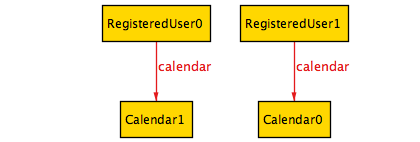
\includegraphics[width=0.6\textwidth]{../Alloy/noInteration.png}
    \caption{No interaction model}
     \label{fig:noint}
     \end{figure}
   \end{center} 
\chapter*{Time Reporting}
\begin{tabularx}{\linewidth}{|r|X|X|}
  \hline  & {\bf Paolo Polidori} & {\bf Marco Edemanti}\\
  \hline RASD writing & 19 hours & 19 hours\\
  \hline RASD revision & 1 hours & 0 hours\\
  \hline
\end{tabularx}\\
\listoffigures
\lstlistoflistings
\end{document}